\documentclass[a4paper, 14pt]{extarticle}

% Поля
%--------------------------------------
\usepackage{geometry}
\geometry{a4paper,tmargin=2cm,bmargin=2cm,lmargin=3cm,rmargin=1cm}
%--------------------------------------


%Russian-specific packages
%--------------------------------------
\usepackage[T2A]{fontenc}
\usepackage[utf8]{inputenc} 
\usepackage[english, main=russian]{babel}
%--------------------------------------

\usepackage{textcomp}

% Красная строка
%--------------------------------------
\usepackage{indentfirst}               
%--------------------------------------             


%Graphics
%--------------------------------------
\usepackage{graphicx}
\graphicspath{ {./images/} }
\usepackage{wrapfig}
%--------------------------------------

% Полуторный интервал
%--------------------------------------
\linespread{1.3}                    
%--------------------------------------

%Выравнивание и переносы
%--------------------------------------
% Избавляемся от переполнений
\sloppy
% Запрещаем разрыв страницы после первой строки абзаца
\clubpenalty=10000
% Запрещаем разрыв страницы после последней строки абзаца
\widowpenalty=10000
%--------------------------------------

%Списки
\usepackage{enumitem}

%Подписи
\usepackage{caption} 

%Гиперссылки
\usepackage{hyperref}

\hypersetup {
	unicode=true
}

%Рисунки
%--------------------------------------
\DeclareCaptionLabelSeparator*{emdash}{~--- }
\captionsetup[figure]{labelsep=emdash,font=onehalfspacing,position=bottom}
%--------------------------------------

\usepackage{tempora}

%Листинги
%--------------------------------------
\usepackage{listings}
\lstset{
  basicstyle=\ttfamily\footnotesize, 
  %basicstyle=\footnotesize\AnkaCoder,        % the size of the fonts that are used for the code
  breakatwhitespace=false,         % sets if automatic breaks shoulbd only happen at whitespace
  breaklines=true,                 % sets automatic line breaking
  captionpos=t,                    % sets the caption-position to bottom
  inputencoding=utf8,
  frame=single,                    % adds a frame around the code
  keepspaces=true,                 % keeps spaces in text, useful for keeping indentation of code (possibly needs columns=flexible)
  keywordstyle=\bf,       % keyword style
  numbers=left,                    % where to put the line-numbers; possible values are (none, left, right)
  numbersep=5pt,                   % how far the line-numbers are from the code
  xleftmargin=25pt,
  xrightmargin=25pt,
  showspaces=false,                % show spaces everywhere adding particular underscores; it overrides 'showstringspaces'
  showstringspaces=false,          % underline spaces within strings only
  showtabs=false,                  % show tabs within strings adding particular underscores
  stepnumber=1,                    % the step between two line-numbers. If it's 1, each line will be numbered
  tabsize=2,                       % sets default tabsize to 8 spaces
  title=\lstname                   % show the filename of files included with \lstinputlisting; also try caption instead of title
}
%--------------------------------------

%%% Математические пакеты %%%
%--------------------------------------
\usepackage{amsthm,amsfonts,amsmath,amssymb,amscd}  % Математические дополнения от AMS
\usepackage{mathtools}                              % Добавляет окружение multlined
\usepackage[perpage]{footmisc}
%--------------------------------------

%--------------------------------------
%			НАЧАЛО ДОКУМЕНТА
%--------------------------------------

\begin{document}

%--------------------------------------
%			ТИТУЛЬНЫЙ ЛИСТ
%--------------------------------------
\begin{titlepage}
\thispagestyle{empty}
\newpage


%Шапка титульного листа
%--------------------------------------
\vspace*{-60pt}
\hspace{-65pt}
\begin{minipage}{0.3\textwidth}
\hspace*{-20pt}\centering

\includegraphics[width=\textwidth]{emblem}
\end{minipage}
\begin{minipage}{0.67\textwidth}\small \textbf{
\vspace*{-0.7ex}
\hspace*{-6pt}\centerline{Министерство науки и высшего образования Российской Федерации}
\vspace*{-0.7ex}
\centerline{Федеральное государственное бюджетное образовательное учреждение }
\vspace*{-0.7ex}
\centerline{высшего образования}
\vspace*{-0.7ex}
\centerline{<<Московский государственный технический университет}
\vspace*{-0.7ex}
\centerline{имени Н.Э. Баумана}
\vspace*{-0.7ex}
\centerline{(национальный исследовательский университет)>>}
\vspace*{-0.7ex}
\centerline{(МГТУ им. Н.Э. Баумана)}}
\end{minipage}
%--------------------------------------

%Полосы
%--------------------------------------
\vspace{-25pt}
\hspace{-35pt}\rule{\textwidth}{2.3pt}

\vspace*{-20.3pt}
\hspace{-35pt}\rule{\textwidth}{0.4pt}
%--------------------------------------

\vspace{1.5ex}
\hspace{-35pt} \noindent \small ФАКУЛЬТЕТ\hspace{80pt} <<Информатика и системы управления>>

\vspace*{-16pt}
\hspace{47pt}\rule{0.83\textwidth}{0.4pt}

\vspace{0.5ex}
\hspace{-35pt} \noindent \small КАФЕДРА\hspace{50pt} <<Теоретическая информатика и компьютерные технологии>>

\vspace*{-16pt}
\hspace{30pt}\rule{0.866\textwidth}{0.4pt}
  
\vspace{11em}

\begin{center}
\Large {\bf Лабораторная работа № 2} \\ 
\large {\bf по курсу <<Языки и методы программирования>>} \\
\large <<Разработка простейшего класса на языке Java>> 
\end{center}\normalsize

\vspace{8em}


\begin{flushright}
  {Студент группы ИУ9-21Б Горбунов А. Д. \hspace*{15pt}\\ 
  \vspace{2ex}
  Преподаватель Посевин Д. П.\hspace*{15pt}}
\end{flushright}

\bigskip

\vfill
 

\begin{center}
\textsl{Москва 2023}
\end{center}
\end{titlepage}
%--------------------------------------
%		КОНЕЦ ТИТУЛЬНОГО ЛИСТА
%--------------------------------------

\renewcommand{\ttdefault}{pcr}

\setlength{\tabcolsep}{3pt}
\newpage
\setcounter{page}{2}

\section{Задание}\label{Sect::task}
Выполнение лабораторной работы заключается в составлении на языке Java одного из
классов, приведённых в таблице. В классе обязательно должны присутствовать конструктор и метод toString.
Отладку разработанного класса необходимо осуществить в методе main
вспомогательного класса Test. Использование контейнерных классов из стандартной библиотеки языка Java не разрешается.
Класс n-мерных вещественных векторов с операциями сложения, вычитания и нормализации. Любая операция должна возвращать новый вектор, оставляя исходные вектора нетронутыми.

\section{Результаты}\label{Sect::res}

Исходный код программы представлен в листинге~\ref{lst:code1}, ~\ref{lst:code2}, ~\ref{lst:code3}.

\begin{figure}[!htb]
\begin{lstlisting}[language={},caption={класс Test},label={lst:code1}]
import java.util.Scanner;
public class Test {
    static int n = 4;
    public static void main(String[] args) {
        double[] arr_1 = new double[n];
        arr_1[0] = 5; arr_1[1] =3; arr_1[2]=1;
        Vector vec_1 = new Vector(n, arr_1);
        Vector vec_2 = new Vector(n, arr_1);
        System.out.println("vec_1:");
        vec_1.printVector();
        System.out.println("vec_2:");
        vec_2.printVector();
        Vector vec_new_1 = vec_1.sum(vec_2);
        System.out.println("vec_new_1 = vec_1.sum(vec_2):");
        vec_new_1.printVector();
        System.out.println("vec_1:");
        vec_1.printVector();
        System.out.println("vec_2:");
        vec_2.printVector();

        Vector vec_new_2 = vec_1.subtraction(vec_2);
        System.out.println("vec_new_2 = vec_1.subtraction(vec_2):");
        vec_new_2.printVector();
        System.out.println("vec_1:");
        vec_1.printVector();
        System.out.println("vec_2:");
        vec_2.printVector();
\end{lstlisting}
\end{figure}

\begin{figure}[!htb]
\begin{lstlisting}[language={},caption={класс Test(продолжение)},label={lst:code2}]
        Vector vec_new_3 = vec_new_1.normalization();
        System.out.println("vec_new_3 = vec_new_1.normalization() :");
        vec_new_3.printVector();
        System.out.println("vec_new_1:");
        vec_new_1.printVector();
        /////////////////////////////////////////////////
        Scanner scan = new Scanner(System.in);
        double[] arr_2 = new double[n];
        double[] arr_3 = new double[n];

        for(int i = 0; i < n; i++)
        {
            if(scan.hasNextDouble())
                arr_2[i] = scan.nextDouble();
            else
            {
                System.out.println("Error");
                break;
            }
        }
        Vector vec_3 = new Vector(n, arr_2);

        for(int i = 0; i < n; i++)
        {
            if(scan.hasNextDouble())
                arr_3[i] = scan.nextDouble();
            else
            {
                System.out.println("Error");
                break;
            }
        }
        Vector vec_4 = new Vector(n, arr_3);
        System.out.println("vec_3:");
        vec_3.printVector();
        System.out.println("vec_4:");
        vec_4.printVector();
        Vector vec_sum_vec_1__vec_3 = vec_3.sum(vec_4);
        System.out.println("vec_sum_vec_1__vec_3:");
        vec_sum_vec_1__vec_3.printVector();

    }
}
\end{lstlisting}
\end{figure}

\begin{figure}[!htb]
\begin{lstlisting}[language={},caption={класс Vector},label={lst:code3}]
import static java.lang.Math.*;
public class Vector {
    static private int n;
    private double[] coordinates;
    public Vector(int n, double[] coordinates)
    {
        this.n = n;
        this.coordinates = new double[this.n];
        for(int i = 0; i < n;i++)
            this.coordinates[i] = 0;
        for(int i = 0; i < coordinates.length;i++)
            this.coordinates[i] = coordinates[i];
    }
    public Vector sum(Vector vec_2)
    {
        double[] sup_coordinates = new double[this.n];
        for(int i = 0; i < n; i++)
            sup_coordinates[i] = coordinates[i] + vec_2.coordinates[i];
        Vector new_vec = new Vector(sup_coordinates.length, sup_coordinates);
        return new_vec;
    }
    public Vector subtraction(Vector vec_2)
    {
        double[] sup_coordinates = new double[this.n];
        for(int i = 0; i < n; i++)
            sup_coordinates[i] = coordinates[i] - vec_2.coordinates[i];
        Vector new_vec = new Vector(sup_coordinates.length, sup_coordinates);
        return new_vec;
    }
    public Vector normalization()
    {
        double[] sup_coordinates = new double[this.n];
        double size = size();
        for(int i = 0; i < n; i++)
            sup_coordinates[i] = coordinates[i]/size;
        Vector new_vec = new Vector(sup_coordinates.length, sup_coordinates);
        return new_vec;
    }
    public double size()
    {
        double sum = 0;
        for(int i = 0; i < n; i++)
            sum += this.coordinates[i] * this.coordinates[i];
        return sqrt(sum);
    }
    public void printVector()
    {
        for(int i = 0; i < n; i++)
            System.out.println(i + 1 +". " + coordinates[i]);
        System.out.println();
    }

    
} 
\end{lstlisting}
\end{figure}

\begin{figure}[!htb]
Результат запуска представлен на рисунке ~\ref{fig:picture_1.png}, ~\ref{fig:picture_2.png}, ~\ref{fig:picture_3.png}.
\end{figure}

\begin{figure}[!htb]
	\centering
	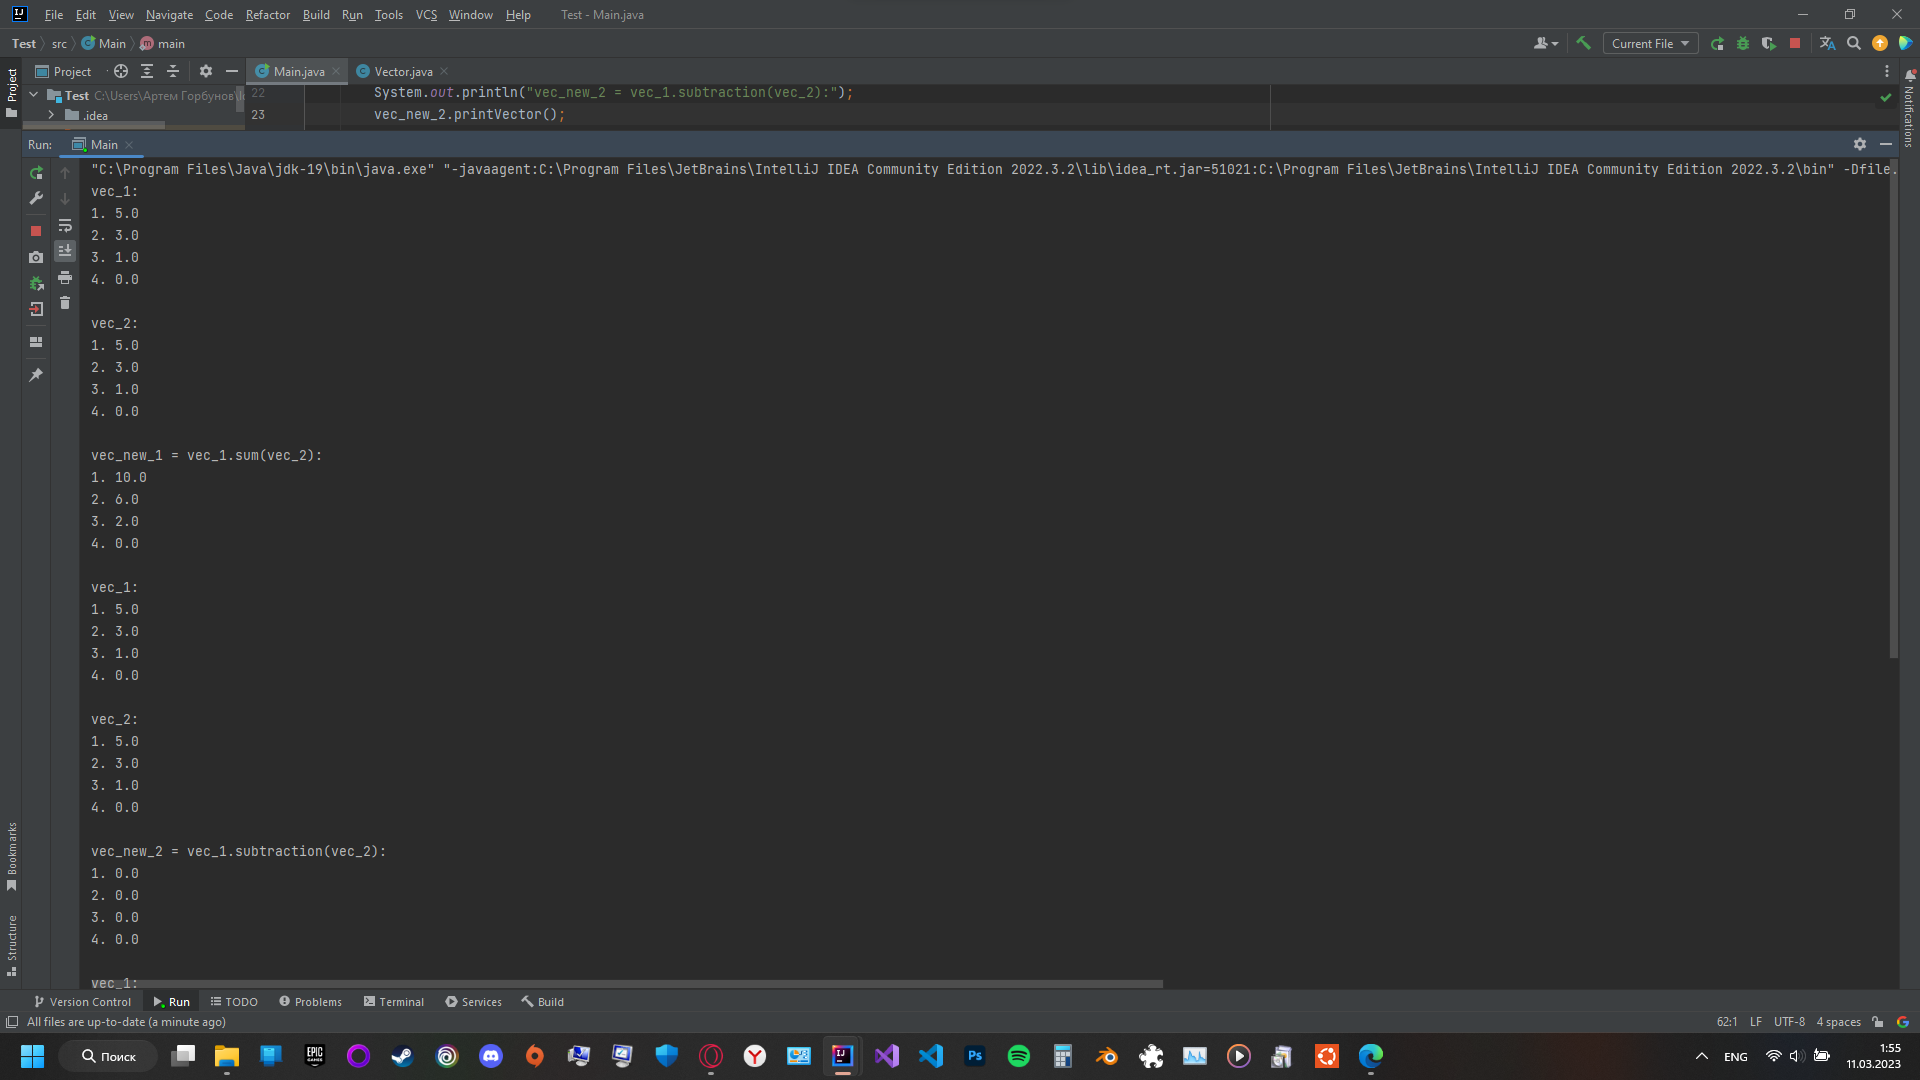
\includegraphics[width=0.8\textwidth]{picture_1.png}
\caption{Вывод программы}
\label{fig:picture_1.png}
\end{figure}

\begin{figure}[!htb]
	\centering
	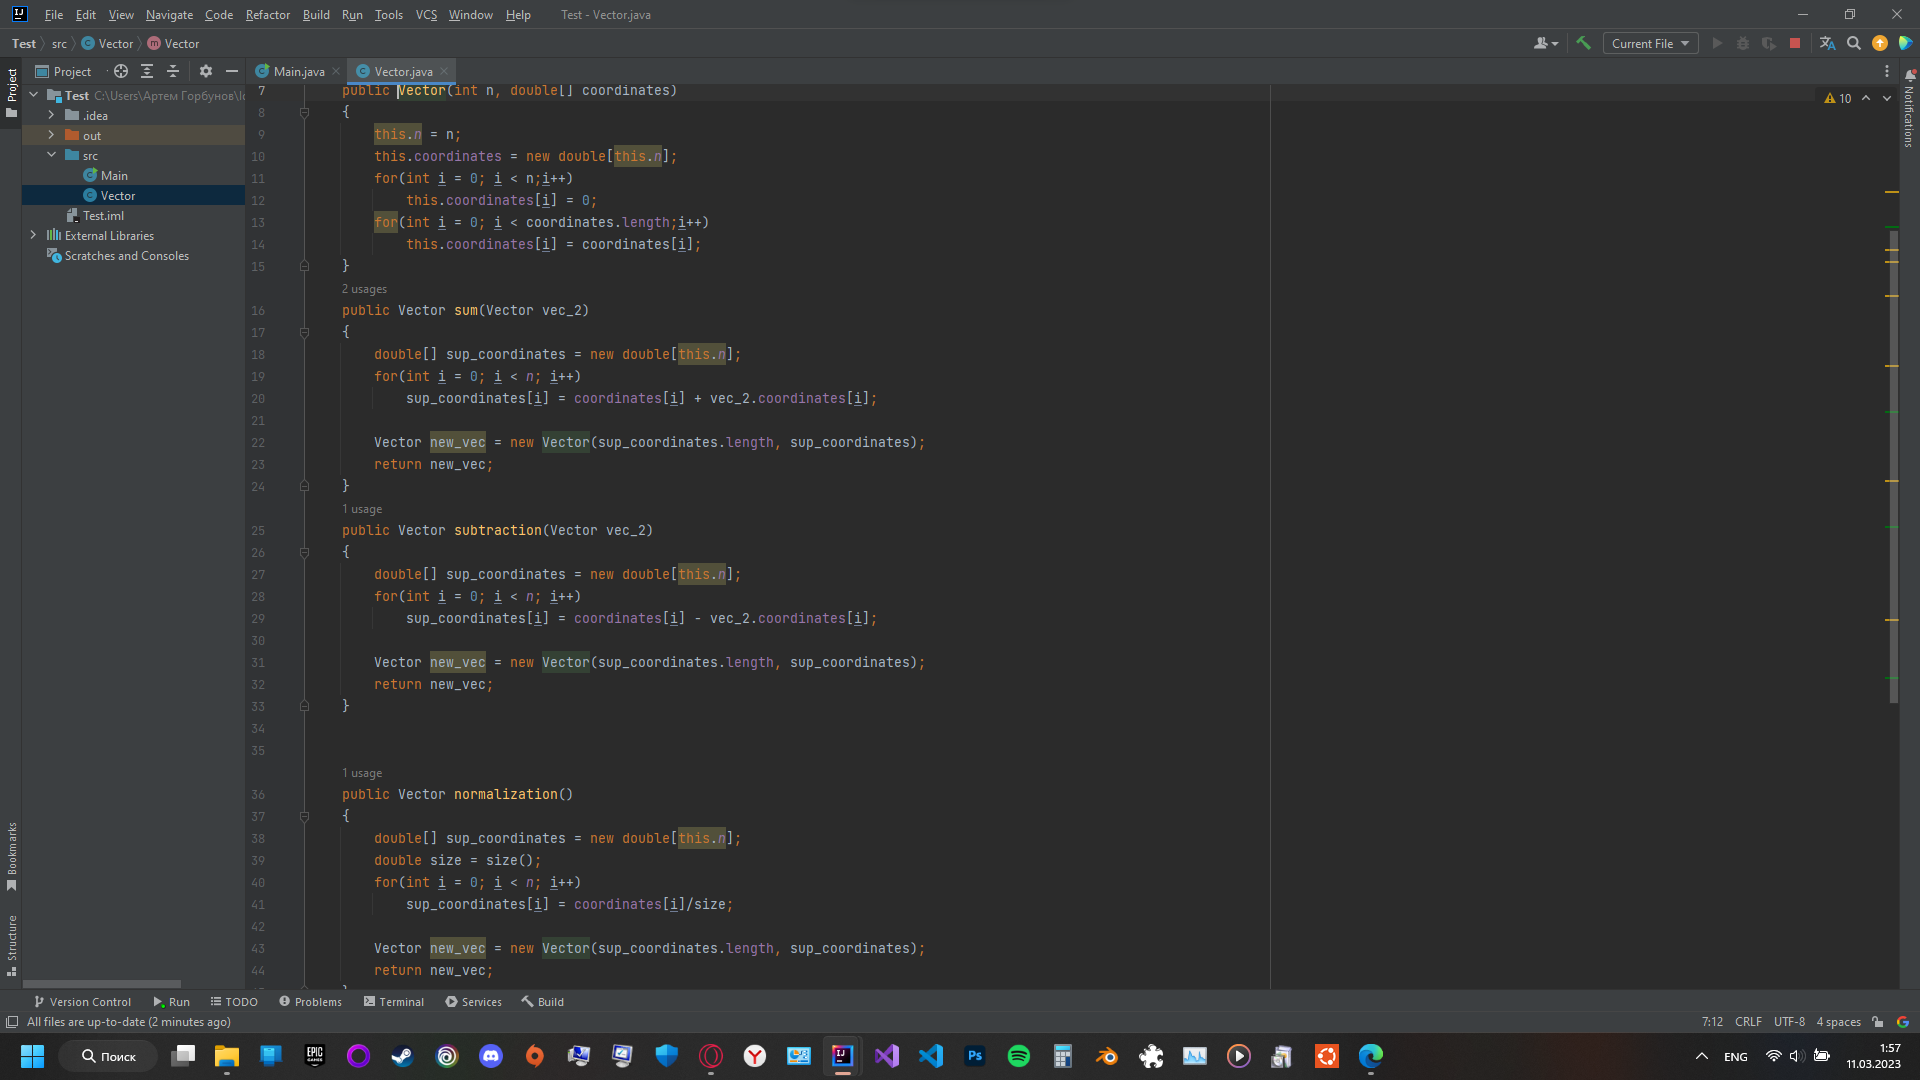
\includegraphics[width=0.8\textwidth]{picture_2.png}
\caption{Работа программы}
\label{fig:picture_2.png}
\end{figure}

\begin{figure}[!htb]
	\centering
	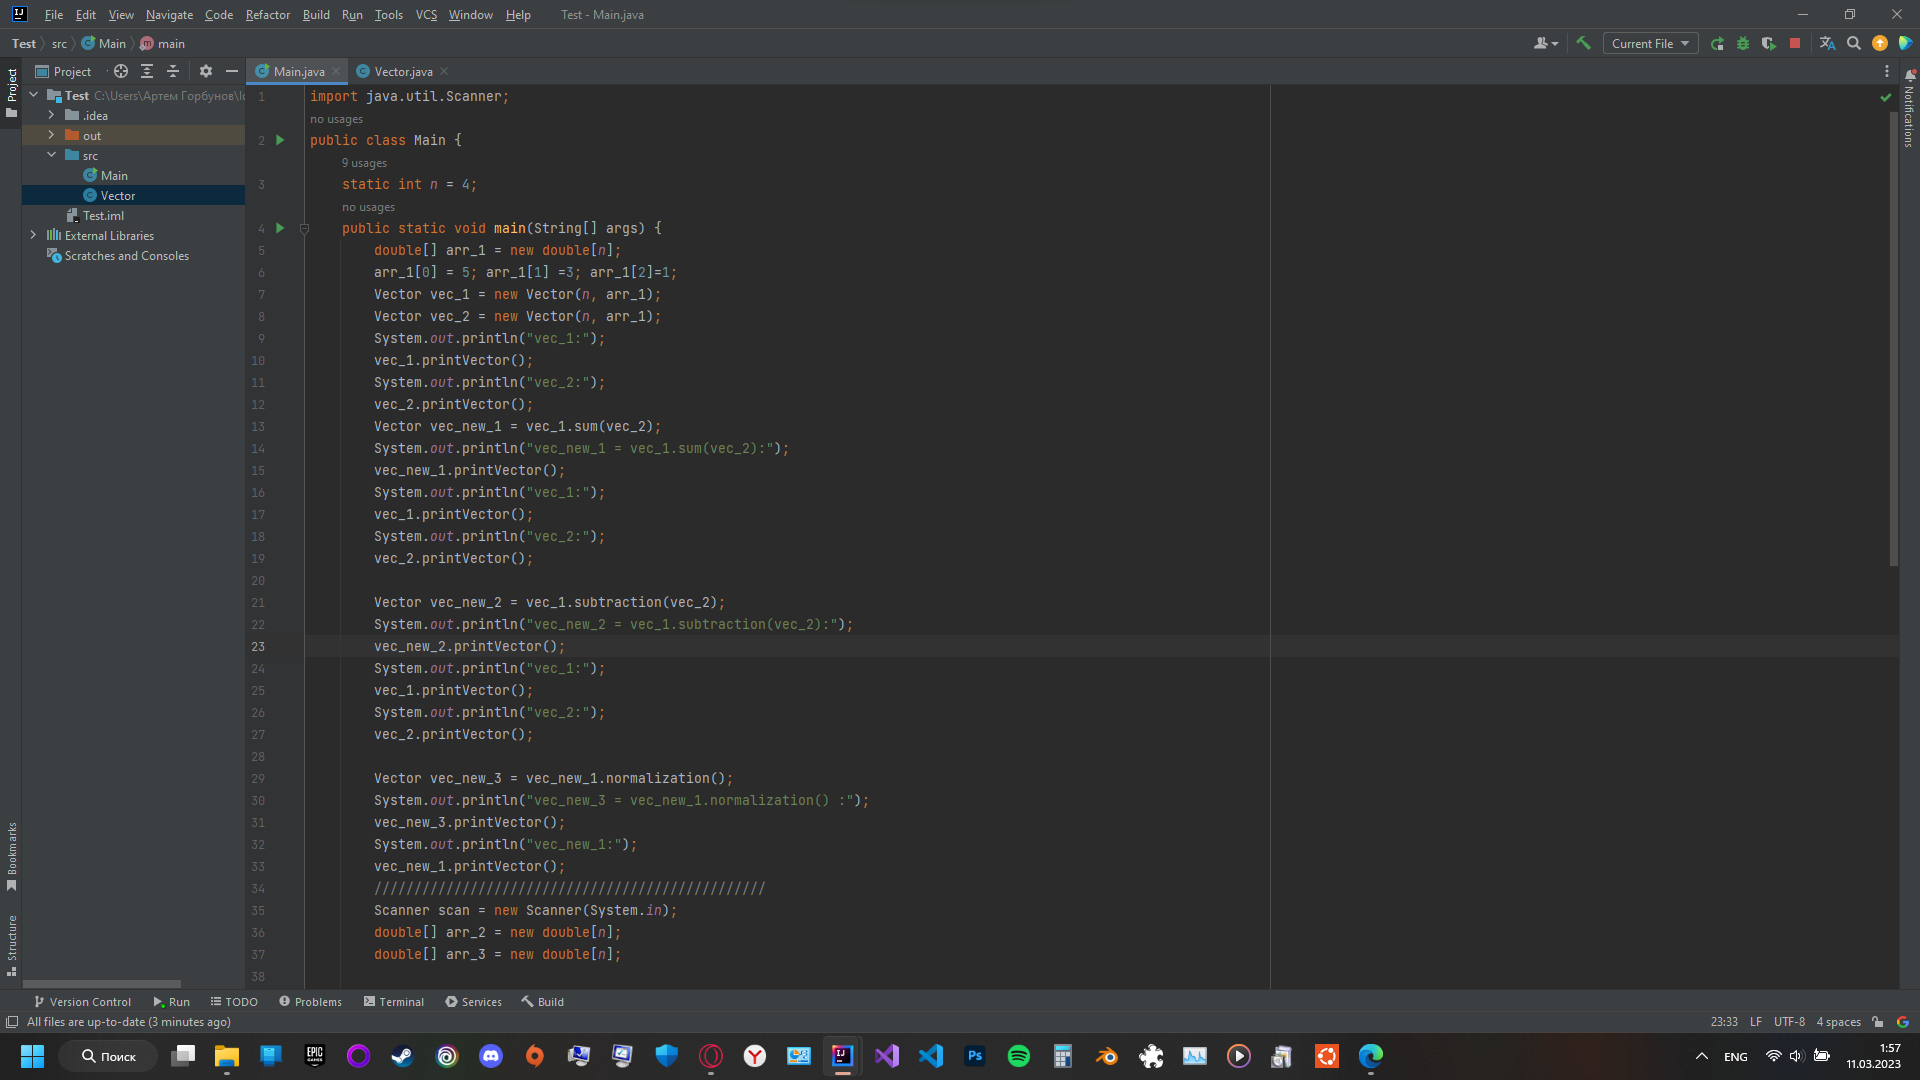
\includegraphics[width=0.8\textwidth]{picture_3.png}
\caption{Работа программы}
\label{fig:picture_3.png}
\end{figure}

\end{document}

